\clearpage
\chapter{IMPLEMENTATION ET RESULTATS}

\textbf{Introduction}\par
Ce chapitre se concentre sur l'implémentation des résultats de notre projet, en mettant en lumière les performances des modèles et les résultats obtenus à partir de nos expériences. Nous présenterons une analyse détaillée des performances de chaque modèle utilisé, en mettant en évidence les forces et les faiblesses de chacun. En outre, nous effectuerons une comparaison approfondie des résultats obtenus, en examinant les métriques de performance clés telles que la précision, le rappel et la F-mesure. Cette section offrira un aperçu complet des résultats de notre projet d'analyse des sentiments, en fournissant des informations précieuses sur l'efficacité de nos approches et sur les leçons apprises tout au long du processus d'implémentation.

\section{Environement de travail et les outils }
\subsection{Langague de programmation}
Nous avons utilisé le langage de programmation\textbf{\textit{ Python}} comme principal outil de développement en raison de sa syntaxe simple et lisible, son caractère open source qui lui confère une utilisation libre, ses riches bibliothèques spécialisés comme ScikitLearn, les outils interactifs comme Jupyter Notebooks facilitant l’expérimentation et le prototypage rapide.
Python se démarque comme un choix idéal pour le déploiement des modèles d’apprentissage automatique d’une manière efficace car il permet aux développeurs de se focaliser sur leurs taches plutôt que sur les détails de mis en œuvre.      

\subsection{Environnement de développement}

%%%%%%%%%%%%% JUPYTER %%%%%%%%%%
\subsubsection{Jupyter Notebook}
Le langage de programmation Python est utilisé dans de plusieurs IDE. Pour ce projet nous avons choisi l'IDE Jupyter Notebook,  étant une application web open source et qui est utilisée pour créer et partager des documents contenant du code, des équations, des visualisations et du texte. \par
Dans le cadre de l'installation de Jupyter, nous avons opté pour la distribution Anaconda. Cette distribution propose un ensemble d'outils particulièrement pertinents pour les Data Scientists, qui leur permettent de tirer pleinement parti de la puissance impressionnante de Python. Outre sa gratuité et son caractère open source, Anaconda simplifie le processus de travail grâce à son accessibilité accrue. L'installation des bibliothèques dans l'environnement Anaconda suffit pour les rendre opérationnelles et pour coder sur Jupyter. \par
Les packages contenus dans la distribution Anaconda sont compatibles avec Windows, Linux et MacOS. Parmi les packages les plus populaires et couramment employés, on retrouve numpy, scipy, sklearn, keras, TensorFlow, opencv, matplotlib, entre autres. Au cours de ce projet, nous avons principalement travaillé avec les trois derniers packages mentionnés.
%%%%%%%%%%%%%%%%%%%% VS CODE %%%%%%%%%%%%
\subsubsection{Visual Studio Code }
Pour la programmation de l’interface web on a utilisé Visual Studio Code, souvent abrégé VS Code, qu’est un éditeur de code source gratuit et open-source développé par Microsoft. Il est largement utilisé par les développeurs de logiciels pour la programmation, l'édition et le débogage de code. VS Code offre de nombreuses fonctionnalités avancées telles que la coloration syntaxique, la complétion automatique, l'intégration avec des systèmes de contrôle de version, des extensions personnalisables, et bien plus encore. Il est disponible sur différentes plateformes, y compris Windows, MacOs et Linux, ce qui en fait un choix populaire pour les développeurs travaillant sur une variété de langages de programmation

%%%%%%%%%%%%%%%%%%%%%%%%ù BIBIOTHEQUES %%%%%%%%%%%

\subsection{Bibliothèques utilisées}


 \textbf{NUMPY}\footnote{\href{https://numpy.org/}{https://numpy.org/}} est la bibliothèque open-source fondamentale du calcul scientifique en Python pour le traitement de tableaux à usage général (voir le logo dans la figure ci- dessous). Elle fournit des tableaux multidimensionnels de haute performance et des outils pour les manipuler. \par
 Au-delà de ses nombreuses utilisations dans le cadre scientifique, Numpy peut aussi être utilisée en tant que conteneur multidimensionnel performant pour des données générales. Ce qui rend NumPy accessible et productif est sa syntaxe de haut niveau, sa large variété de fonctions mathématiques complètes et de générateurs de nombres aléatoires ainsi que sa capacité de prise en charge d’un large éventail de plateformes matérielles et informatiques. 
 \par
 
\textbf{PANDAS}
\footnote{\href{https://pandas.pydata.org/}{https://pandas.pydata.org/}} est une bibliothèque open source de Python, largement utilisée pour la manipulation et l'analyse de données. Développée initialement par Wes McKinney en 2008, Pandas offre des structures de données flexibles et expressives, principalement les DataFrames et les Series, permettant des opérations rapides et faciles sur des ensembles de données tabulaires et des séries chronologiques. \par

\textbf{MATPLOTLIB} \footnote{\href{https://matplotlib.org/}{https://matplotlib.org/}} est une bibliothèque de visualisation de données en Python qui offre une vaste gamme de graphiques pour représenter visuellement des données. Créée par John D. Hunter en 2003, Matplotlib est particulièrement prisée pour sa capacité à générer des graphiques statiques, animés et interactifs de haute qualité.\par

\textbf{SEABORN}\footnote{\href{https://seaborn.pydata.org/}{https://seaborn.pydata.org/}} est une bibliothèque de visualisation de données basée sur Matplotlib. Elle est conçue pour rendre les graphiques statistiques plus attrayants et plus faciles à créer. Seaborn simplifie la création de visualisations complexes et est particulièrement bien adaptée pour travailler avec des données structurées comme les DataFrames de Pandas.\par 

\textbf{NLTK}\footnote{\href{https://www.nltk.org/}{https://www.nltk.org/}} (Natural Language ToolKit) est une collection de modules de programmes open-source, de didacticiels et d’ensembles de problèmes permettant de créer des programmes pour l’analyse de texte. Ce kit a été à l’origine créé par Steven Bird et Edward Loper en conjonction avec des cours de linguistique computationnelle à l’université de Pennsylvanie en 2001.\par
NLTK inclut le traitement statistique du langage naturel et est lié à des corpus labélisés. Joint à la librairie, NTLK offre des tutoriels, des échantillons de données, des démonstrations graphiques ainsi qu’une documentation complète sur l’interface de programmation API.\par


\textbf{Scikit-learn}, souvent abrégé en "sklearn", est une bibliothèque open source en Python spécialisée dans le domaine de l'apprentissage automatique (machine Learning). Elle propose une large gamme d'algorithmes et d'outils pour la création, l'entraînement et l'évaluation de modèles de machine Learning. Cette bibliothèque vise à rendre l'apprentissage automatique plus accessible grâce à des interfaces conviviales et cohérentes.
Scikit-learn est reconnue pour sa simplicité et sa modularité. Elle couvre différents types d'apprentissage, tels que la classification, la régression, le regroupement (clustering), la réduction de dimension, la détection d'anomalies, et bien plus encore. Elle propose une grande variété d'algorithmes populaires, notamment les machines à vecteurs de support (SVM), les forêts aléatoires, les k-plus proches voisins (KNN), la régression linéaire, et bien d'autres.
En outre, scikit-learn fournit des outils pour la préparation des données, l'évaluation des performances des modèles et la validation croisée. Cette bibliothèque est largement utilisée par les professionnels du machine learning en raison de sa documentation complète, de sa grande communauté et de son intégration aisée avec d'autres bibliothèques Python telles que Numpy, pandas et matplotlib.

\textbf{TensorFlow} \footnote{\href{https://www.tensorflow.org/?hl=fr}{https://www.tensorflow.org/?hl=fr}} est une plateforme d’apprentissage automatique open source de bout en bout (voir le logo dans la figure ci-dessous). Il est doté d’un écosystème exhaustif et flexible de bibliothèques, de ressources et d’outils communautaires permettant aux chercheurs de promouvoir les avancées de l’apprentissage automatique, et aux développeurs de créer et de déployer aisément des applications d’apprentissage automatique.\par
 TensorFlow a vu le jour aux mains d’ingénieurs et de chercheurs membres de l’équipe Google Brain au sein de l’organisation de recherche sur l’intelligence artificielle de Google. TensorFlow fournit des API Python et C++ statistiques, ainsi qu’une API rétro compatible non cautionnée pour d’autres langages. \par

\textbf{Keras} \footnote{\href{https://keras.io/}{https://keras.io/}}  est une bibliothèque de haut niveau pour le développement et l'entraînement de modèles de réseaux de neurones profonds. Initialement développée par François Chollet, Keras est maintenant intégrée au sein de la bibliothèque TensorFlow de Google, mais elle peut également être utilisée avec d'autres backends comme Theano ou CNTK. \par

\textbf{Djanjo}\footnote{\href{https://www.djangoproject.com/}{https://www.djangoproject.com/}} est un framework web de haut niveau écrit en Python qui permet le développement rapide et facile de sites web robustes et sécurisés. Créé par Adrian Holovaty et Simon Willison en 2003, Django est conçu pour aider les développeurs à prendre des applications du concept à la réalisation aussi rapidement que possible.

%%%%%%%% Présentation DES CORPUS %%%%%%%%%%%%%%%%
\section{Présentation des corpus} 
Les ensembles de données utilisées dans ce projet ont été extraits de Kaggle \footnote{\href{https://www.kaggle.com/} {https://www.kaggle.com/}}.  La plateforme fournit des jeux de données, des notebooks et des didacticiels gratuits dont les scientifiques de données ont besoin pour réaliser leurs projets d'apprentissage automatique \cite{kaggle_wiki}. 

%%%%%%%%%%%%%%%ù SENTIMENTs DATA %%%%%%%%%%%%%%%
\subsection{Sentiment140-MV }
Le dataset des sentiments également connu sous le nom  \textit{Sentiment140-MV} \footnote{\href{https://www.kaggle.com/datasets/kamyab20/sentiment140mv} {https://www.kaggle.com/datasets/kamyab20/sentiment140mv}}, est un ensemble de données largement utilisé dans le domaine de l'analyse des sentiments. Il comprend des tweets collectés à partir de Twitter, annotés avec l'étiquette du sentiment correspondant, généralement positif et négatif.  
Chaque entrée de données a les caractéristiques suivantes :
\begin{itemize}
    \item {\textbf{ Ids:}} un nombre entier qui représente l'id du tweet;
    \item {\textbf{Date:}} le timestamp du tweet; \par
    \item {\textbf{ Flag:}}  la requête qui a été utilisée pour récupérer le Tweet avec Twitter API. S'il n'y a pas de requête, cette valeur est NO QUERY. 
    \item {\textbf{Utilisateur:}} le nom de l’utilisateur qui a publié le message;
    \item {\textbf{ texte:}} le contenu réel du tweet.
\end{itemize}

La figure [\ref{fig:figure8}]  montre l'apparence du jeu de données Sentiment140-MV avant toute opération supplémentaire effectuée sur celui-ci.


\begin{figure}[h]
    \centering
    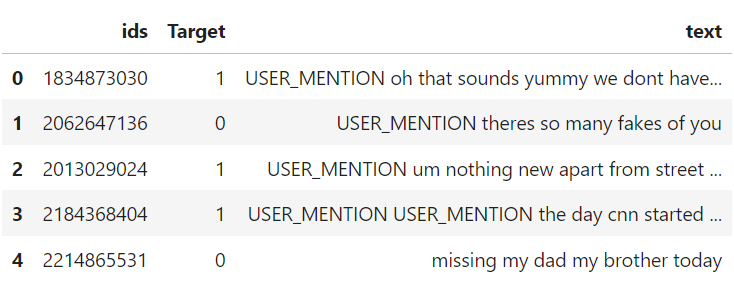
\includegraphics[width=0.7\textwidth]{project_report/figures/Dataset-APRES.png} 
    \caption{Sentiment140-MV dataset originale. }
        \label{fig:figure8}
 
\end{figure}

%%%%%%%%%%%%%%%% EMOTIONS DATA %%%%%%%%%%%%%%%%
\subsection{Emotions}
Le dataset \textit{Emotions}\footnote{\href{https://www.kaggle.com/datasets/nelgiriyewithana/emotions} {https://www.kaggle.com/datasets/nelgiriyewithana/emotions}} est une collection de messages en anglais provenant de Twitter, minutieusement annotés avec six émotions fondamentales: la colère, la peur, la joie, l'amour, la tristesse et la surprise. Ce dataset constitue une ressource précieuse pour comprendre et analyser le spectre diversifié des émotions exprimées dans les textes courts sur les réseaux sociaux. Chaque entrée dans ce dataset se compose d'un segment de texte représentant un message Twitter et d'une étiquette correspondante indiquant l'émotion prédominante transmise. Les émotions sont classées en six catégories : la tristesse (0), la joie (1), l'amour (2), la colère (3), la peur (4) et la surprise (5).

La figure [\ref{fig:figEm}]  montre l'apparence du jeu de données Emotionq avant toute opération supplémentaire effectuée sur celui-ci.

\begin{figure}[h]
    \centering
    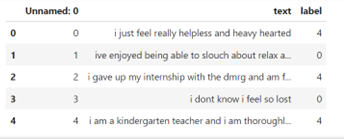
\includegraphics[width=0.7\linewidth]{project_report/figures/emotion.png}
    \caption{Emotions dataset originale.}
    \label{fig:figEm}
\end{figure}




Une analyse descriptive a été effectuée pour mieux comprendre les ensembles de données et obtenez des informations à ce sujet. Il est rapporté dans la section suivante avec une analyse exploratoire des données et quelques astuces de pré-traitement pour réduire le bruit des données.




%%%%%%%%%%%%%%%%%ù ANALYSE DES SENTIMENTS %%%%%%%%
\section{Analyse des sentiments}
Un flux précis a été suivi pour exécuter les expériences, afin d'éviter d'introduire \textit{Bias} dus à des exécutions non structurées. À partir de l'ensemble de données brut, les données
ont été pré-traitées en supprimant les hashtags, les mentions, les ponctuations et les mots d'arrêt, pour réduire les données non informatives, réduisant ainsi la taille globale des données pour gérer, accélérer les expériences.  toutes les lettres et les mots sont changés en lettres de cas inférieures \textit{(Lower-case)} pour assurer l'uniformité. En outre, les phrases ont été divisées en mots individuels, ou des jetons en utilisant le Tokeniser de NLTK. 
le processus est le même pour tout nos modules. Chaque séquence des deux corpus passe par les mêmes étapes de prétraitement.  

%%%%%%%%%%%%%%%%%%% ANALYSE EXPLORATOIRE %%%%%%%%%%%%%

\subsection{Analyse éxploratoire}


\begin{figure}[h]
    \centering
    \includegraphics[width=0.6\linewidth]{project_report/figures/WhatsApp Image 2024-06-07 à 20.42.44_c32b6e6d.jpg}
    \caption{Distribution des classes dans l'ensemble des données Sentiment140-MV.}
    \label{fig:figDes}
\end{figure}

%%%%%%%%%%%%%%%%%%%%%%%%%%%%%%%%%%%%%%%%%%%%%%%%%%%%%
19 995 messages étiquetés sont disponibles, ils sont soit positifs soit négatifs et les deux classes ne  sont pas équilibrées comme le montre l figure [\ref{fig:figDes}]. Cela a été fait exprès par les créateurs du jeu de données pour limiter les complexités liées aux classes déséquilibrées, ce qui simplifie ainsi les phases suivantes. 




%%%%%%%%%%%%%%%%%%%%%%%%%%%%%%%%%%%%%%%%%%%%%%%%%
%%%%%%%%%%%%%% Statistique du dataset %%%%%%%%%%%



\begin{table}[h!]
    \centering
    \begin{tabular}{>{\raggedright\arraybackslash}p{0.6\linewidth}>{\centering\arraybackslash}p{0.3\linewidth}}
        \textbf{Statistique} & \textbf{Valeur} \\
        Nombre moyen de caractères : & 73 \\
        \multicolumn{2}{c}{\rule{0.8\linewidth}{0.4pt}} \\
        Tweet le plus long : & 157 caractères \\
        \multicolumn{2}{c}{\rule{0.8\linewidth}{0.4pt}} \\
        Tweet le plus court : & 3 caractères \\
        \multicolumn{2}{c}{\rule{0.8\linewidth}{0.4pt}} \\
        Nombre de caractères, quantile 0,99 : & 134 \\
        \multicolumn{2}{c}{\rule{0.8\linewidth}{0.4pt}} \\
        Nombre moyen de mots : & 14 \\
        \multicolumn{2}{c}{\rule{0.8\linewidth}{0.4pt}} \\
        Tweet le plus long : & 33 mots \\
        \multicolumn{2}{c}{\rule{0.8\linewidth}{0.4pt}} \\
        Tweet le plus court: & 1 mot \\
        \multicolumn{2}{c}{\rule{0.8\linewidth}{0.4pt}} \\
        Nombre de mots, quantile 0,99 : & 28 \\
        \multicolumn{2}{c}{\rule{0.8\linewidth}{0.4pt}} \\
        Nombre de mots uniques : & 18835 \\
    \end{tabular}
    \caption{Statistiques du jeu de données}
    \label{tab:dataset_statistics}
\end{table}
%%%%%%%%%%%%%%%%%%%%%%%%%%%%%%%%%%%%%%%%%%%%%%%%%%%ù

Pour comprendre l'effet du pré-traitement, une analyse quantitative a été réalisée avant de prendre toute mesure sur le corpus. Les statistiques clés concernant la longueur des Tweets sont résumées ici dans le tableau [\ref{tab:dataset_statistics}]. 

%%%%%%%%%%%%%%%%%%%%%%%% PRE-TRAITEMENT %%%%%%%%%%%



\subsection{Nettoyage des données} 
Dans la phase de nettoyage des données, un processus rigoureux a été entrepris pour garantir la qualité et la cohérence du jeu de données. Tout d'abord, les lignes en double ont été identifiées et éliminées, permettant ainsi d'assurer l'intégrité des enregistrements. De plus, dans le souci de ne conserver que les informations essentielles pour l'analyse ultérieure, seules les colonnes pertinentes ont été préservées. Parmi celles-ci figuraient les identifiants uniques associés à chaque entrée, la variable cible indiquant la polarité sentimentale (positif ou négatif), ainsi que le texte brut des messages eux-mêmes. Cette approche sélective a non seulement simplifié le jeu de données, mais a également facilité les étapes suivantes d'analyse et de modélisation.
%%%%%%%%%%%%%%% TABLE %%%%%%%%%%%%%%%%ùù
\begin{table}[h!]
    \centering
    \begin{tabular}{lll}
        \toprule
        \textbf{Variable} & \textbf{Avant nettoyage} & \textbf{Après nettoyage} \\
        \midrule
        Nombre d'entrées & 19995 & 18213 \\
        Nombre de colonnes & 6 & 3 \\
        Types de données & \texttt{int64 (2), object (1)} & \texttt{int64 (4), object (2)} \\
        Doublons & 1782 & - \\
        \midrule
        \textbf{Cible} & & \\
        Positif & 11628 & - \\
        Négatif & 6585 & - \\
        \bottomrule
    \end{tabular}
    \caption{Caractéristiques du jeu de données avant et après le nettoyage}
    \label{tab:data_summary}
\end{table}
Le tableau [\ref{tab:data_summary}] fournit un résumé des données avant et après le processus de nettoyage, mettant en évidence le nombre d'enregistrements avant le nettoyage ainsi que le nombre de lignes dupliquées identifiées.


\newpage

%%%%%%%%%%%%%%%%%%%%%%%%%%%%%%%
\subsection{Préparation des données}
Au cours de prétraitement des données, nous avons utilisé deux méthodes : lemmatisation et le stemming, la première consiste à réduire les mots à leurs formes de base en utilisant des règles heuristiques simple, tandis que la deuxième utilise des règles linguistiques pour transformer les mots en leurs lemme correct.
L’utilisation des deux méthodes a produit des résultats similaires, ce qui s’explique par le contexte limité du dataset des sentiments avec peu de variations morphologiques et grammatical, par conséquence les transformations nécessaires pour réduire ces formes sont minimales.

\subsection{Représentation textuelle}
%%%%%%%%%%%%%%%%%%%ù TABLE %%%%%%%%%%%%%%%%%%%%%%
\begin{table}[h!]
    \centering
    \begin{tabular}{lcccccccc}
        \toprule
        & \multicolumn{4}{c}{CountVectorizer} \\
        \cmidrule(lr){2-5}
        Métriques & Accuracy & Précision & Recall & F1-score \\
        \midrule
        RL & 89\% & 90\% & 93\% & 91\% \\
        CNB & 85\% & 89\% & 87\% & 88\% \\
        MNB & 84\% & 85\% & 91\% & 88\% \\
        \bottomrule
    \end{tabular}
    \caption{Performances des modèles avec CountVectorizer}
    \label{tab:model_performance_countvectorizer}
\end{table}

\begin{table}[h!]
    \centering
    \begin{tabular}{lcccccccc}
        \toprule
        & \multicolumn{4}{c}{TF-IDF vectorizer} \\
        \cmidrule(lr){2-5}
        Métriques & Accuracy & Précision & Recall & F1-score \\
        \midrule
        RL & 87\% & 87\% & 94\% & 90\% \\
        CNB & 84\% & 86\% & 89\% & 88\% \\
        MNB & 78\% & 75\% & 98\% & 85\% \\
        \bottomrule
    \end{tabular}
    \caption{Performances des modèles avec TF-IDF vectorizer}
    \label{tab:model_performance_tfidfvectorizer}
\end{table}

Pour la représentation textuelle, deux méthodes ont été introduites ; TF-IDF et     CountVectorizer. Cette dernière est la méthode la plus simple pour créer des vecteurs, elle compte le nombre des mots dans un document, Il ne prend pas en compte l'importance relative des mots dans le corpus. En revanche TF-IDF (Term Frequency-Inverse Document Frequency) prend en compte à la fois la fréquence des termes dans un document (TF) et l'inverse de la fréquence des documents dans lesquels un terme apparaît (IDF)
Pour l’analyse préliminaire des données, nous avons utilisé la régression logistique, la naïve Bayes multinomial et la naïve Bayes complément comme algorithmes de base en raison de leur simplicité, de leur rapidité et aussi leurs faibles besoins en calcul.
TF-IDF a donné des résultats moins performants que CountVectorizer, cela peut être dû à   la simplicité et l’efficacité de comptage brut des occurrences qui semble mieux s’adapter avec les caractéristiques spécifiques de ce dataset.







 
%%%%%%%%%% DIVISION DES DONNEES %%%%%%%%%%%%%%%%%
\subsection{Division des données}
Dans cette étape, nous avons procédé à la division des données en ensembles d'entraînement, de validation et de test, en suivant une approche adaptée à chaque type de modèle : les modèles de machine learning et les modèles de deep learning.

Pour les modèles de machine learning traditionnels, tels que les SVM, Naive Bayes et Régression Logistique, nous avons simplement divisé les données en un ensemble d'entraînement et un ensemble de test. L'ensemble d'entraînement a été utilisé pour entraîner le modèle, tandis que l'ensemble de test a été réservé pour évaluer la performance du modèle final sur des données non vues.

Pour les modèles de deep learning, en raison de leur complexité et de leur tendance à sur-ajuster aux données, nous avons effectué une division plus fine en trois ensembles : un ensemble d'entraînement, un ensemble de validation et un ensemble de test. L'ensemble d'entraînement a été utilisé pour entraîner le modèle, l'ensemble de validation a été utilisé pour ajuster les hyperparamètres et surveiller la performance pendant l'entraînement, et l'ensemble de test a été utilisé pour évaluer la performance finale du modèle sur des données non vues.

Les deux tableaux suivants présentent les résultats obtenus lors de la division des données en différentes tailles pour les modèles de régression logistique et de complément naïf bayésien. 

%%%%%%%%%%%%%%%%%%%%%% TABLE %%%%%%%%%%%%%%%%%%%
\begin{table}[h!]
    \centering
    \caption{\textit{Performances du modèle RL}}
    \begin{tabular}{lcccc}
        \toprule
        Test\_size & Accuracy & Recall & Précision & F1\_score \\
        \midrule
        0.1 & 0.87 & 0.94 & 0.86 & 0.90 \\
        0.2 & 0.87 & 0.94 & 0.87 & 0.90 \\
        0.3 & 0.86 & 0.94 & 0.86 & 0.90 \\
        0.4 & 0.87 & 0.94 & 0.86 & 0.89 \\
        \bottomrule
    \end{tabular}
\end{table}

\begin{table}[h!]
    \centering
    \caption{\textit{Performance du modèle CNB}}
    \begin{tabular}{lcccc}
        \toprule
        Test\_size & Accuracy & Recall & Précision & F1\_score \\
        \midrule
        0.1 & 0.87 & 0.94 & 0.86 & 0.90 \\
        0.2 & 0.85 & 0.87 & 0.89 & 0.88 \\
        0.3 & 0.86 & 0.94 & 0.86 & 0.90 \\
        0.4 & 0.87 & 0.94 & 0.86 & 0.89 \\
        \bottomrule
    \end{tabular}
\end{table} 
\newpage

Dans la lumière de ces résultats, on observe que peu de changements significatifs sont remarqués dans les performances des modèles, ce qui suggère que la division des données en différentes tailles de test n'a pas un impact considérable sur les performances des modèles de régression logistique et de complément naïf bayésien. Cela indique une certaine robustesse des modèles par rapport à la variation de la taille des données de test. Il est également important de noter que, malgré les légères fluctuations observées dans les métriques de performance telles que l'accuracy, le recall, la précision et le F1-score, les performances générales des modèles restent relativement stables sur différentes divisions des données. Ces résultats sont encourageants car ils suggèrent que les modèles sont capables de généraliser efficacement sur de nouveaux ensembles de données, ce qui est essentiel pour assurer leur utilité dans des applications réelles. Cependant, il convient de poursuivre l'exploration de ces modèles sur d'autres jeux de données et de considérer d'autres facteurs pouvant influencer leurs performances, tels que la qualité et la quantité des données d'entraînement.


%%%%%%%%%%% CLASSIFICATION %%%%%%%%%%%% 
\subsection{La classification}
Pour cette tâche d’analyse des sentiments et de classification en positive et négative sur le jeu de données sentiment140-MV, nous avons utilisé des algorithmes d’apprentissage automatique supervisé tels que :
\begin{itemize}
    \item Régression logistique
    \item Naïve Bayes multinomial
    \item Naïve Bayes complément
    \item Adaboost
    \item NuSVC
    \item RNN-LSTM
\end{itemize}

La performance des modelés créés à l’aide de ces classificateurs est évaluée en calculant l’accuracy, la précision, le recall, et le F1-score, ainsi en visualisant la matrice de confusion et les graphiques de performance pour les réseaux de neurones.   
%%%%%%%%%%%%%%%%%%%%%% RESULTATS %%%%%%%

\subsection{Résultats et discussion }
%%%%%%%%%%%%%%%%%%%%%%%%%% TABLE %%%%%%%%%%%
\begin{table}[h!]
    \centering
    \begin{tabular}{lcccc}
        \toprule
        \textbf{Classificateur} & \textbf{Accuracy} & \textbf{Precision} & \textbf{Recall} & \textbf{F1-score} \\
        \midrule
        Model 1 : RNN\_LSTM & 85\% & 85\% & 85\% & 85\% \\
        Modèle 2 : MNB & 78\% & 82\% & 78\% & 85\% \\
        Modèle 3 : CNB & 85\% & 85\% & 85\% & - \\
        Modèle 4 : RL & 87\% & 88\% & 88\% & 87\% \\
        Modèle 5 : AdaBoost & 80\% & 81\% & 80\% & 81\% \\
        Model 6 : Nu-SVC & 87\% & 88\% & 88\% & 88\% \\
        \bottomrule
    \end{tabular}
    \caption{Performance des classificateurs}
    \label{tab:classifier_performance}
\end{table}

%%%%%%%%%%%%%%%%%%%%%%%%%%%%%%%%%%%%%%%%%%%%%
Le modele Naïve Bayes multinomial est moins performant en comparaison avec les autres modèles ; bien que le MNB soit simple et rapide à entrainer, il suppose l’indépendance conditionnelle entre les caractéristiques ce qui n’est pas entièrement applicable aux données textuelles, aussi il est moins performant sur les datasets ou les classes sont déséquilibrés parce qu’il est basé sur le fréquence brute dans les calculs des probabilités. \par
\begin{figure}[h]
    \centering
    \begin{minipage}{0.45\textwidth}
        \centering
        \includegraphics[width=0.8\textwidth]{project_report/figures/complementNB_sentimentçmatrice.png}
        \caption{\textit{Matrice de confusion du modèle CNB}.}
        \label{fig:figureSHJJJR}
    \end{minipage}\hfill
    \begin{minipage}{0.45\textwidth}
        \centering
        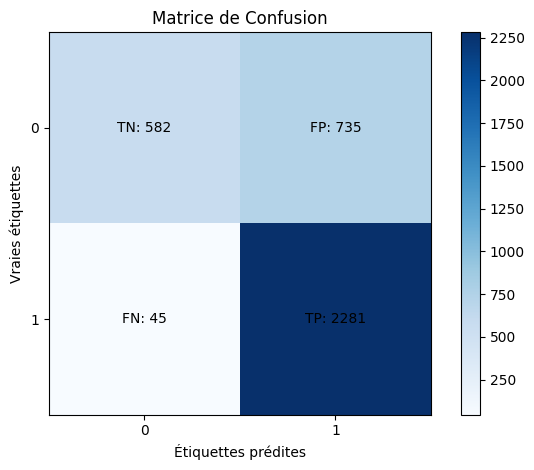
\includegraphics[width=0.8\textwidth]{project_report/figures/multinomial NB_sentiment_matrice.png}
        \caption{\textit{Matrice de confusion du modèle MNB }.}
        \label{fig:figureNBVV}
    \end{minipage}
\end{figure} 


Concernant le modele Naïve Bayes complément est parmi les algorithmes les plus performant sur ce dataset des sentiments en notant sa rapidité, cela s’explique par le fait CNB est performant sur les jeux donnés déséquilibrés comme dans notre cas où il fonctionne en ajustant la manière dont les probabilités sont calculées pour tenir compte des données manquants par rapport à d’autre classes (basé sur la fréquence complément).\par
\begin{figure}[h]
    \centering
    \begin{minipage}{0.45\textwidth}
        \centering
        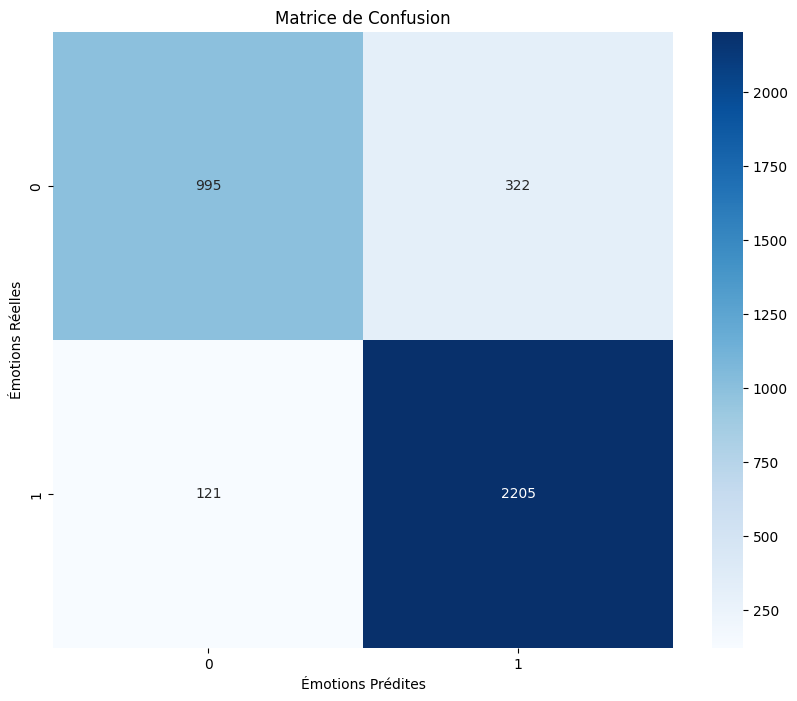
\includegraphics[width=0.8\textwidth]{project_report/figures/matrice_sentimnt-NUSVC.png}
        \caption{\textit{Matrice de confusion du modèle nu-SVC}.}
        \label{fig:figureSHJJJR}
    \end{minipage}\hfill
    \begin{minipage}{0.45\textwidth}
        \centering
        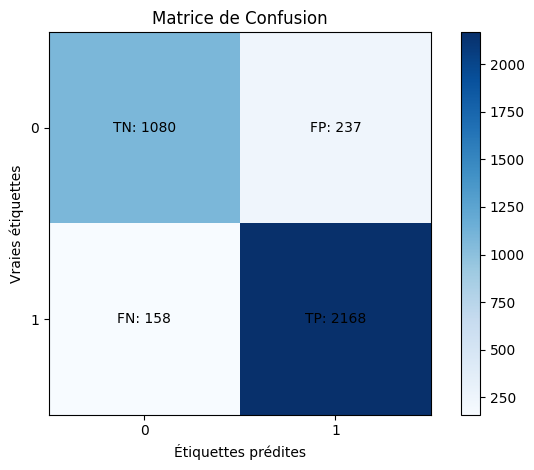
\includegraphics[width=0.8\textwidth]{project_report/figures/RL_sentiment_matrice.png}
        \caption{\textit{Matrice de confusion du modèle RL }.}
        \label{fig:figureNBVV}
    \end{minipage}
\end{figure} 
Pour NuSVC et la régression logistique, ces modèles ont réussi à capturer efficacement les relations entre les caractéristiques des données et des classes des sentiments leurs efficacité peut être attribuée à leur capacité à modéliser des frontières de décision complexes tout en maintenant une interprétabilité raisonnable ce qui en fait des choix attrayants pour les applications de classifications.\par
\begin{figure}[h]
    \centering
    \begin{minipage}{0.45\textwidth}
        \centering
        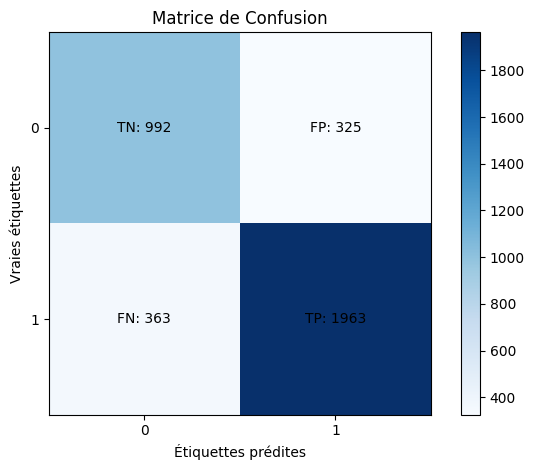
\includegraphics[width=0.8\textwidth]{project_report/figures/adaboost_sentiment_matrice.png}
        \caption{\textit{Matrice de confusion du modèle AdaBoost}.}
        \label{fig:figureSHJJJR}
    \end{minipage}\hfill
    \begin{minipage}{0.45\textwidth}
        \centering
        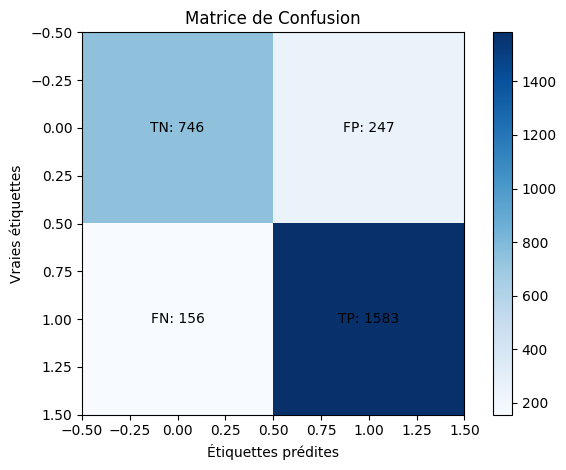
\includegraphics[width=0.8\textwidth]{project_report/figures/RNN_sentiment_matrice.png}
        \caption{\textit{Matrice de confusion du modèle RNN-LSTM}.}
        \label{fig:figureNBVV}
    \end{minipage}
\end{figure} 

Pour Adaboost, les performances sont moyennes par rapport à d’autre modèles, il a démontré une capacité à améliorer progressivement la précision de la classification en agrégeant plusieurs classificateurs faibles, cependant son efficacité peut être limitée dans des cas ou les données sont déséquilibrées où lorsque les caractéristiques discriminantes sont difficiles à extraire ce qui peut entrainer une performance moins satisfonte par rapport à d’autre modèles.\par


Bien que le modèle RNN-LSTM ait produit des résultats solides, il moins performant que des modèles tels que NusSVC et la régression logistique dans ce cas en raison de plusieurs facteurs ; la performance des modèles peut être influencée par la qualité des données d'entraînement, et la répartition déséquilibré des classes qui pose un défi lors de la création de modèle, car les algorithmes ont tendance à favoriser les classes majoritaires et peuvent avoir des performances médiocres pour les classes minoritaires.   




%%%%%%%%%%%%%%%%%%ù ANALYSE DES EMOTIONS %%%%%%%%%%%%

\section{Analyse des émotions}
\subsection{Analyse éxploratoire}

\begin{figure}[h]
    \centering
    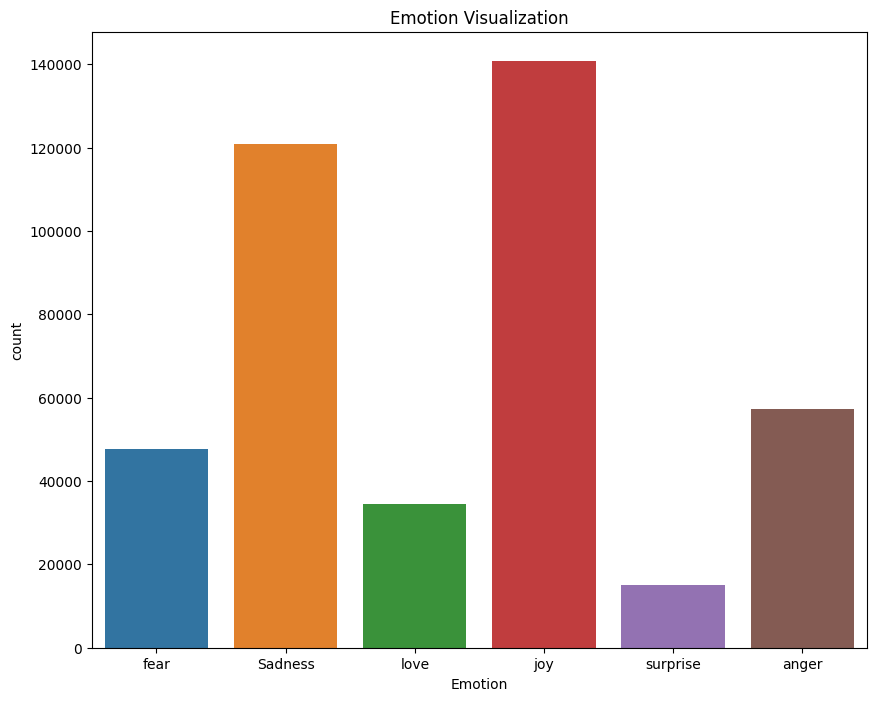
\includegraphics[width=0.7\linewidth]{project_report/figures/repartition-emotion.png}
    \caption{Distribution des classes dans l'ensemble de données Emotions.}
    \label{fig:figDescri}
\end{figure}

%%%%%%%%%%%%%%%%%%%%%%%%%%%%%%%%%%%%%%%%%%%%%%%%%%%%%
Les classes de différentes émotions sont représentées d’une manière inégale, cela signifie plusieurs classes ont beaucoup plus d’exemples que d’autres, créant un déséquilibre significatif. 

\subsection{Nettoyage des données} 
L'étape de nettoyage des données effectuée dans l'analyse des émotions est similaire à celle de l'analyse des sentiments. Dans les deux cas, l'objectif principal est de préparer les données textuelles brutes en éliminant les éléments indésirables et en les rendant prêtes à être analysées par les modèles d'apprentissage automatique ou les techniques d'analyse


\subsection{Préparation des données}
L’application de stemming et lemmatisation sur le dataset des émotions a donné des résultats différents. Lorsque nous avons utilisé la lemmatisation pour le nettoyage des données les performances ont augmenté, tandis que lorsque nous avons appliqué le stemming les performances ont diminué, cela peut s’expliqué par le bon fonctionnement de la lemmatisation qui prend en considération le contexte grammatical et les relations linguistique, par rapport au stemming qu’est moins précis et peut entrainer une perte de sens contextuel et une diminution de performance de modèle utilisé.

\subsection{Représentation textuelle}
Pour le dataset des émotions, l'application des deux techniques de représentation textuelle a donné des résultats différents. L'utilisation de TF-IDF a diminué la performance des modèles par rapport à l'utilisation du vecteur de comptage (CountVectorizer). Cela peut s'expliquer par la nature des émotions, qui sont souvent exprimées par des termes spécifiques. TF-IDF peut diluer l'importance de ces termes en pondérant moins les mots fréquents, ce qui est contre-productif si ces derniers sont précisément ceux qui expriment des émotions importantes. De plus, l'utilisation de bigrammes et de trigrammes a également dégradé la performance des modèles.
%%%%%%%%%%%%%%%%%%%ù TABLE %%%%%%%%%%%%%%%%%%%%%%
\begin{table}[h!]
    \centering
    \caption{Performance des modèles avec CountVectorizer}
    \begin{tabular}{lcccccccc}
        \toprule
        & \multicolumn{4}{c}{CountVectorizer} \\
        \cmidrule(lr){2-5}
        Métriques & Accuracy & Précision & Recall & F1-score \\
        \midrule
        RL & 89\% & 89\% & 89\% & 89\% \\
        CNB & 89\% & 89\% & 89\% & 89\% \\
        MNB & 86\% & 86\% & 86\% & 86\% \\
        \bottomrule
    \end{tabular}
\end{table}

\begin{table}[h!]
    \centering
    \caption{Performance des modèles avec TF-IDF vectorizer}
    \begin{tabular}{lcccccccc}
        \toprule
        & \multicolumn{4}{c}{TF-IDF vectorizer} \\
        \cmidrule(lr){2-5}
        Métriques & Accuracy & Précision & Recall & F1-score \\
        \midrule
        RL & 89\% & 89\% & 89\% & 89\% \\
        CNB & 88\% & 88\% & 88\% & 88\% \\
        MNB & 76\% & 80\% & 73\% & 76\% \\
        \bottomrule
    \end{tabular}
\end{table}
%%%%%%%%%%%%%%%%%%%%%%%%%
\newpage
\subsection{Division des données}
Les résultats obtenus mettent en évidence la stabilité des performances des modèles de régression logistique et de complément naïf bayésien lorsqu'ils sont soumis à des variations de la taille de l'ensemble de test pour le jeu de données sur les émotions. Ces observations indiquent que les modèles conservent une cohérence dans leurs capacités prédictives, peu importe la taille des données de test. Malgré de légères fluctuations dans les métriques d'évaluation telles que l'accuracy, le recall, la précision et le F1-score, les performances globales des deux modèles restent relativement constantes sur différentes tailles d'ensemble de test. Cette constance suggère une certaine robustesse des modèles face aux changements de taille des données de test, ce qui renforce leur capacité à généraliser efficacement sur de nouveaux ensembles de données. En somme, ces résultats démontrent la fiabilité des modèles de régression logistique et de complément naïf bayésien dans leur capacité à maintenir des performances stables et cohérentes, ce qui les rend pertinents pour une utilisation dans divers contextes d'analyse des émotions. 
%%%%%%%%%%%%%%%%%%%ù TABLE %%%%%%%%%%%%%%%%%%%%%%
\begin{table}[h!]
    \centering
    \caption{Modèle de régression logistique}
    \begin{tabular}{lcccc}
        \toprule
        Test\_size & Accuracy & Recall & Précision & F1\_score \\
        \midrule
        0.1 & 0.88 & 0.88 & 0.88 & 0.88 \\
        0.2 & 0.89 & 0.89 & 0.89 & 0.89 \\
        0.3 & 0.89 & 0.89 & 0.89 & 0.89 \\
        0.4 & 0.89 & 0.89 & 0.89 & 0.89 \\
        \bottomrule
    \end{tabular}
\end{table}

\begin{table}[h!]
    \centering
    \caption{Modèle de complément NB }
    \begin{tabular}{lcccc}
        \toprule
        Test\_size & Accuracy & Recall & Précision & F1\_score \\
        \midrule
        0.1 & 0.85 & 0.86 & 0.90 & 0.88 \\
        0.2 & 0.88 & 0.88 & 0.88 & 0.88 \\
        0.3 & 0.85 & 0.86 & 0.90 & 0.88 \\
        0.4 & 0.88 & 0.88 & 0.88 & 0.88 \\
        \bottomrule
    \end{tabular}
\end{table}

\subsection{La classification}
Pour la classification des émotions en plusieurs catégories (joie, amour, colère, surprise, tristesse et peur), nous utilisons des algorithmes d'apprentissage supervisé ainsi que des algorithmes de réseaux de neurones tels que :
\begin{itemize}
    \item Régression logistique;
    \item Naïve Bayes multinomial;
    \item Naïve Bayes complément;
    \item Adaboost;
    \item RNN-LSTM;
    \item CNN.
\end{itemize}
En suivant la même méthodologie d’analyse des sentiments précédente, nous évaluons les classificateurs des émotions en calculant les métriques de performance et en visualisant la matrice de confusion et le graphique des performances pour les réseaux de neurones. \\
Les résultats obtenus à partir des modèles mentionnés seront détaillés dans les sections suivantes, où nous examinerons en profondeur les performances de chaque approche. Chaque modèle sera évalué en fonction de critères tels que la précision, le rappel, la F-mesure et d'autres métriques pertinentes. En outre, nous analyserons les forces et les faiblesses de chaque méthode, en mettant en lumière les aspects clés de leur mise en œuvre et de leur interprétation. Ce niveau de détail permettra une compréhension approfondie des performances de chaque modèle, ainsi que des recommandations pour leur utilisation future dans des scénarios similaires.


\subsection{Résultats et discussion}

%%%%%%%%%%%%%%%%ù TABLE OF RESULTS %%%%%%%%%%%%%%%
\begin{table}[h!]
    \centering
    \caption{Performance des modèles pour le dataset des émotions}
    \label{tab:Em}
    \begin{tabular}{lcccc}
        \toprule
        Dataset des émotions & Accuracy & Precision & Recall & F1-score \\
        \midrule
        Model 1 : RNN\_LSTM & 93\% & 93\% & 93\% & 93\% \\
        Modèle 2 : MNB & 76\% & 80\% & 76\% & 76\% \\
        Modèle 3 : RL & 89\% & 89\% & 89\% & 89\% \\
        Modèle 4 : CNB & 88\% & 88\% & 88\% & 88\% \\
        Modèle 5 : CNN & 93\% & 93\% & 93\% & 93\% \\
        Modèle 6 : AdaBoost & 0.36\% & 24\% & 24\% & 21\% \\
        \bottomrule
    \end{tabular}
\end{table}
%%%%%%%%%%%%%%%%%%%%%%% END OF TABLE %%%%%%%%%%
En se basant sur les résultats obtenus dans les trois modèles (Voir le tableau [\ref{tab:Em}] (Naïve Bayes complément, Naïve Bayes multinomial et la régression logistique), on peut donner les mêmes interprétations obtenues déjà dans le dataset précédent. Cependant, on peut ajouter que le Naïve Bayes complément (CNB) et la régression logistique sont capables de s'adapter à des datasets complexes et volumineux, tout en générant rapidement des résultats en comparaison avec des algorithmes plus lents mais performants.\par
\begin{figure}[h]
    \centering
    \begin{minipage}{0.45\textwidth}
        \centering
        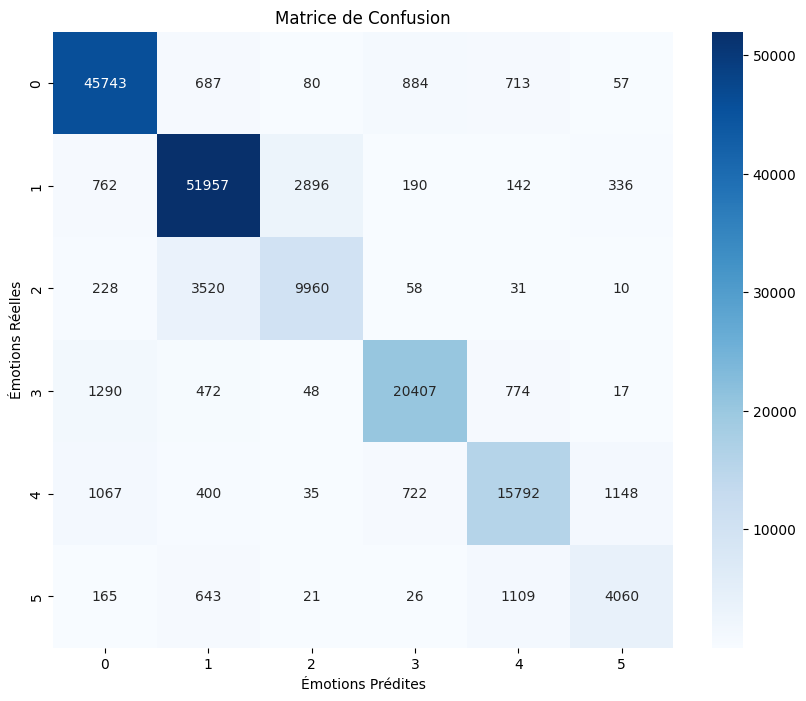
\includegraphics[width=\textwidth]{project_report/figures/matrice-complement NB-emotion.png}
        \caption{\textit{Matrice de confusion du modèle CNB}.}
        \label{fig:figureSHJJJR}
    \end{minipage}\hfill
    \begin{minipage}{0.45\textwidth}
        \centering
        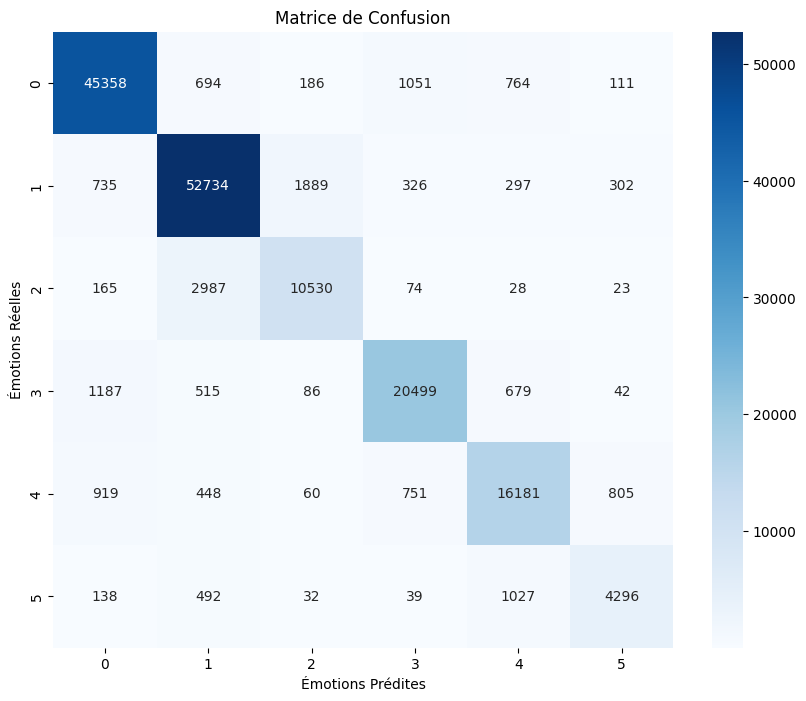
\includegraphics[width=\textwidth]{project_report/figures/RL-matrice-emotion.png}
        \caption{\textit{Matrice de confusion du modèle RL}.}
        \label{fig:figureNBVV}
    \end{minipage}
\end{figure} 


Les performances comparables du CNN et du RNN-LSTM sur le dataset des émotions suggèrent que ces deux architectures sont également efficaces pour traiter ce type de données. Bien que le CNN soit généralement considéré comme plus adapté pour l'extraction de caractéristiques locales à partir de données structurées, et que le RNN-LSTM soit privilégié pour modéliser les dépendances séquentielles à long terme, les résultats montrent que les deux approches sont capables de capturer efficacement les informations pertinentes pour la classification des émotions. Cette observation met en lumière la flexibilité et la robustesse des réseaux de neurones profonds, qui peuvent s'adapter à différents types de données et produire des performances comparables dans des contextes variés.\par
%%%%%%%%%%%%%%ùùùFIG 
\begin{figure}[h]
    \centering
    \begin{minipage}{0.45\textwidth}
        \centering
        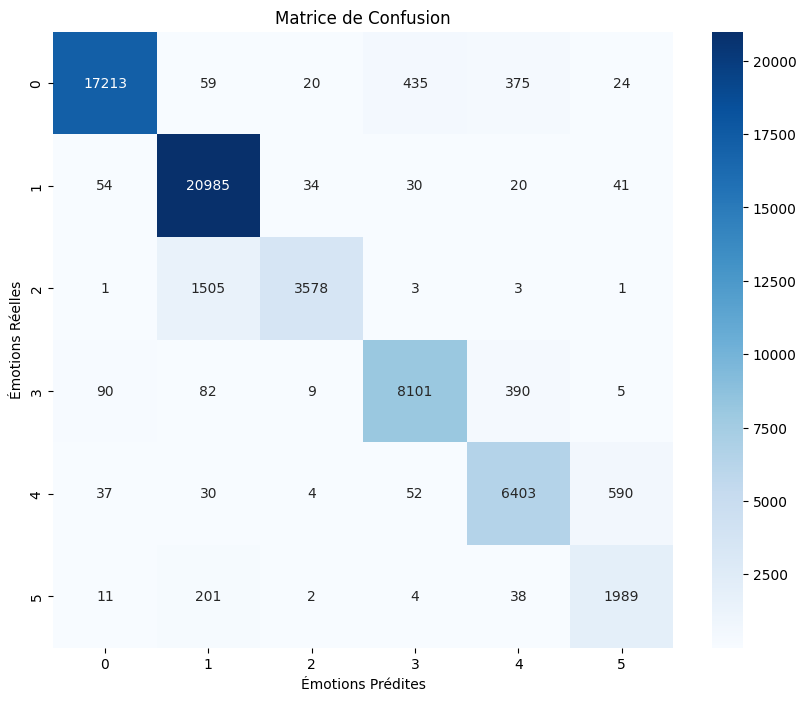
\includegraphics[width=\textwidth]{project_report/figures/CNN_matrice_emotion.png}
        \caption{\textit{Matrice de confusion du modèle CNN}.}
        \label{fig:figureCNN}
    \end{minipage}\hfill
    \begin{minipage}{0.45\textwidth}
        \centering
        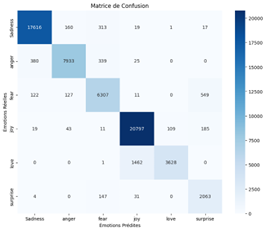
\includegraphics[width=\textwidth]{project_report/figures/emotion_rnn.png}
        \caption{\textit{Matrice de confusion du modèle RNN-LSTM}.}
        \label{fig:figureLSTM}
    \end{minipage}
\end{figure} 



%%%%%%%%%%%%%%%%%FIG 
Malgré l'augmentation du nombre d'estimateurs pour le modèle créé en utilisant le classificateur AdaBoost et l'utilisation de la validation croisée, les performances restent en deçà des attentes.
Cette situation peut être attribuée à plusieurs facteurs, tels que la complexité inhérente des données qui peut rendre l'application de modèles tels qu'AdaBoost mal adaptée, ainsi que le déséquilibre entre les classes.

\begin{figure}[h]
    \centering
    \begin{minipage}{0.45\textwidth}
        \centering
        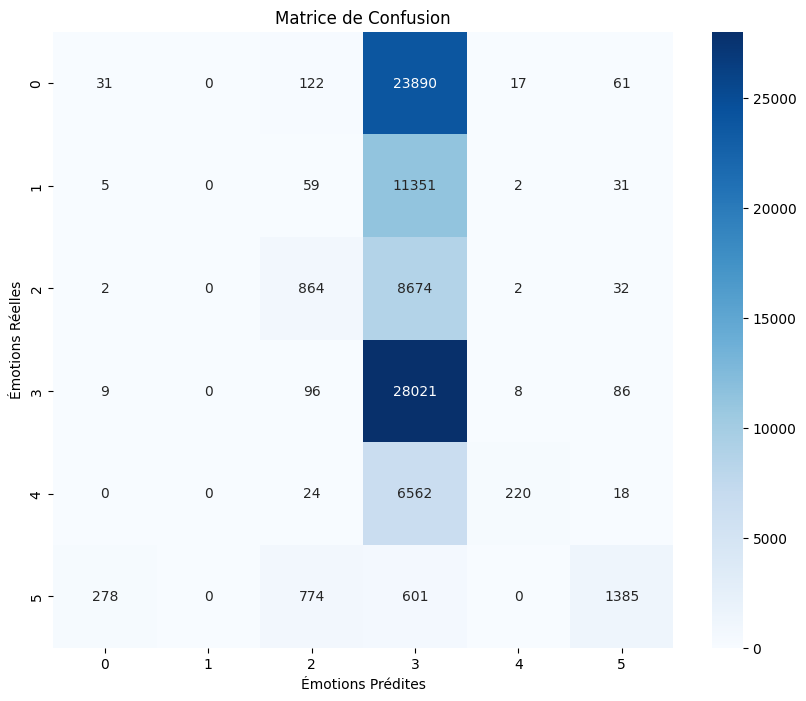
\includegraphics[width=\textwidth]{project_report/figures/adaboost_matrice_emotion.png}
        \caption{\textit{Matrice de confusion du modèle AdaBoost}.}
        \label{fig:figureSHJJJR}
    \end{minipage}\hfill
    \begin{minipage}{0.45\textwidth}
        \centering
        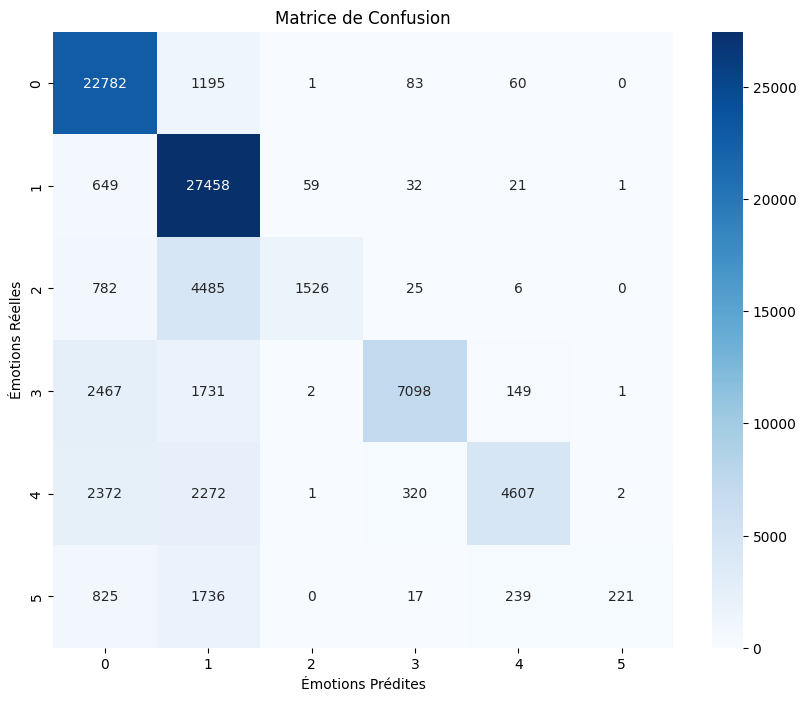
\includegraphics[width=\textwidth]{project_report/figures/multinomial NB-emotion_matrice.png}
        \caption{\textit{Matrice de confusion du modèle MNB}.}
        \label{fig:figureNBVV}
    \end{minipage}
\end{figure} 


\section{Déploiement de l'application}
\subsection{Modélisation}
\textbf{Le langage de Modélisation Unifié UML}
, communément appelé UML, constitue l'un des langages les plus essentiels lorsqu'il s'agit d'initier un projet. Il se révèle être un langage graphique de modélisation fondé sur des symboles graphiques soigneusement élaborés pour offrir une méthode standardisée permettant de visualiser la conception d'un système.
L'UML est employé pour ajuster, représenter, définir et élaborer les documents indispensables à la réalisation réussie d'un projet. Il instaure une norme de modélisation, offrant une représentation architecturale du logiciel. Parmi les divers éléments pouvant être représentés, on compte :
\begin{itemize}
    \item Les activités d'un objet ou d'un logiciel.
    \item Les intervenants (acteurs) du système.
    \item Les processus en cours.
    \item Les schémas de bases de données.
    \item Les éléments constitutifs du logiciel.
    \item La réutilisation de composants existants.
\end{itemize}
Les outils de modélisation UML autorisent même la génération automatique de tout ou partie du code d'une application logicielle, tel que le langage Java, en se basant sur les différents documents conçus.
Pour comprendre l'architecture de notre projet, nous nous sommes servis de deux types de diagramme. La suite explique ceci en détail. \par
\textbf{Diagramme de cas d'utilisation}
\begin{figure}[h]
    \centering
    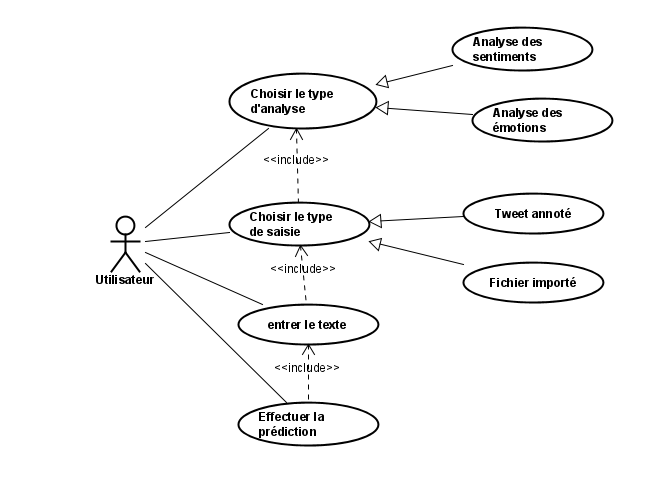
\includegraphics[width=0.7\linewidth]{project_report/figures/Capture d’écran (1208).png}
    \caption{\textit{Diagramme de cas d'utilisation}}
    \label{fig:figUsecase}
\end{figure}
\\Dans un langage UML, les diagrammes de cas d'utilisation modélisent le comportement d'un système et saisissent les exigences de celui-ci. Ils sont utilisés pour décrire le fonctionnement du système et son utilisation par les acteurs, mais sans démontrer comment le système fonctionne à l'interne.
Afin de décrire l'ensemble des fonctions générales et de l'étendue de notre système, nous nous sommes servis du diagramme de cas d'utilisation ci-dessous, qui identifie également les interactions entre le système et ses acteurs.
La Figure [\ref{fig:figUsecase}] présente le schéma global du diagramme de cas d'utilisation de notre système. 


\textbf{Diagramme de séquence}
Les diagrammes de séquence UML sont des outils graphiques d'interaction qui fournissent une vue approfondie sur la manière dont les actions sont exécutées. Ils saisissent l'interrelation entre les objets au sein d'une collaboration donnée. Ces diagrammes ont également une dimension temporelle, mettant en évidence la séquence des interactions par le biais de l'axe vertical du schéma pour représenter le passage du temps, les messages échangés et leur timing respectif. 
La figure [\ref{fig:figsequence}] présente le diagramme de séquence de notre interface :

\begin{figure}[h]
    \centering
    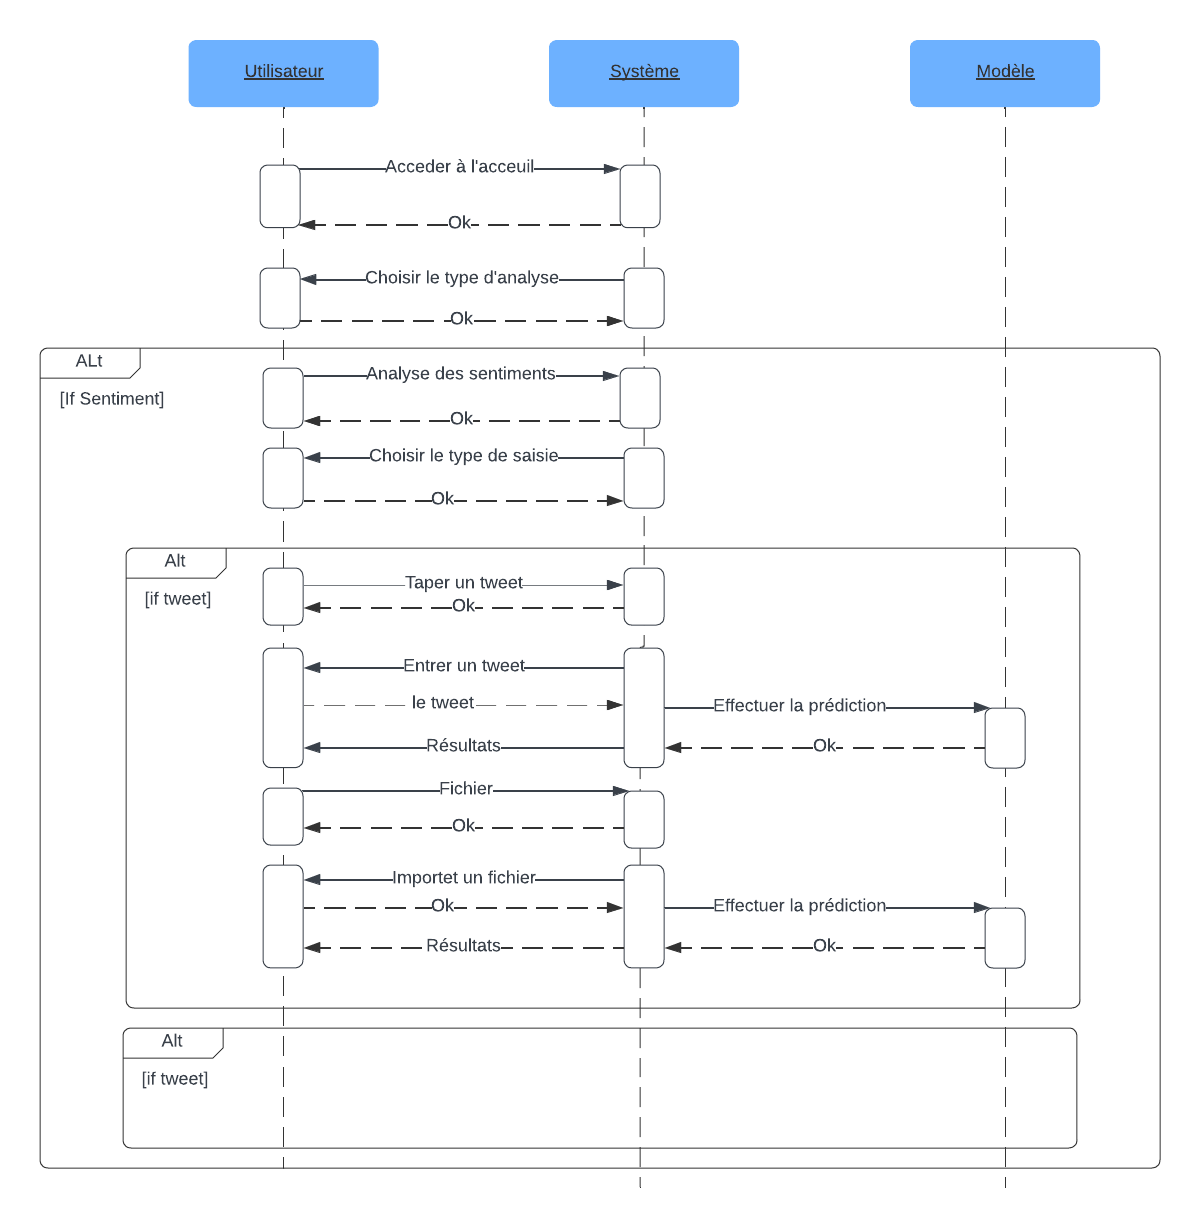
\includegraphics[width=1\linewidth]{project_report/figures/Sequence diagram (3).png}
    \caption{\textit{Diagramme de séquence}}
    \label{fig:figsequence}
\end{figure}


Dans la deuxième partie de l'instruction conditionnelle (else), le processus est similaire à celui précédemment décrit, mais cette fois-ci appliqué à l'identification et au traitement des émotions. Les données sont analysées et catégorisées en fonction des différentes émotions exprimées, suivant une approche semblable à celle utilisée pour les sentiments.
\subsection{Archeticture globale de l'application}
La structure ou l’architecture d'une application définit les schémas et les méthodes employés pour concevoir et élaborer une application. Cette structure fournit un guide ainsi que les procédés recommandés à suivre pour créer une application bien organisée.
Le fonctionnement de notre système global peut être résumé selon les étapes illustrées dans la figure ci-dessous. 
\begin{figure}[h]
    \centering
    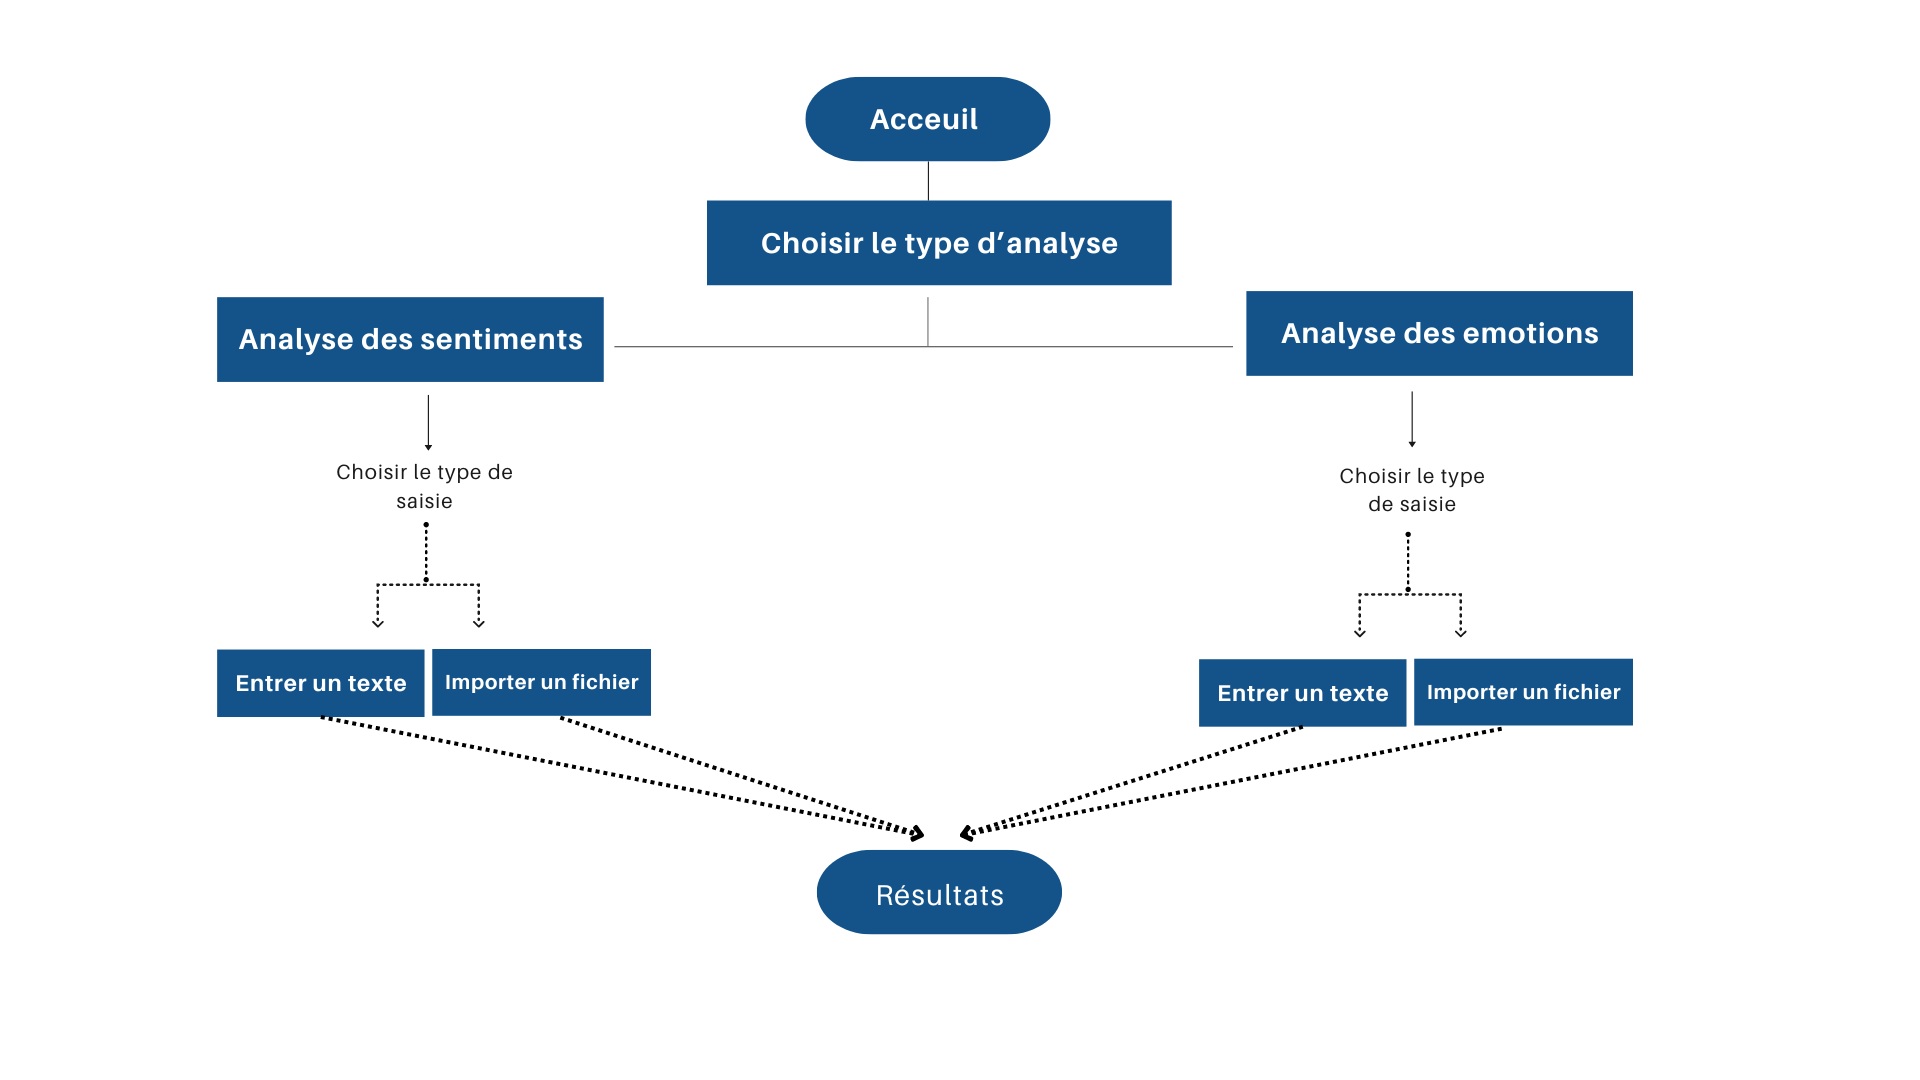
\includegraphics[width=1\linewidth]{project_report/figures/Oui.png}
    \caption{\textit{Archeticture globale de l'application}}
    \label{fig:arch}
\end{figure}
\subsection{Démonstration des interfaces}
\subsubsection{Interface principales}
La première version de cette application permet les fonctionnalités suivantes :
\begin{itemize}
    \item \textbf{Analyse des sentiments et des émotions annotés :} l’application permet aux utilisateurs de taper leurs textes. Une fois le texte est soumis l’application affiche le sentiment ou l’émotion correspondant selon le choix préalable d’utilisateur.
    \item \textbf{Analyse des sentiments et des émotions à partir des fichiers Excel ou csv :} l’application permet aux utilisateurs d’importer des fichiers contenants des tweets, le système analyse ces données et affiche les résultats avec des statistiques.
\end{itemize}
Cette interface [\ref{fig:acc}] ouffre a l'utilisateur la possibilité de choisir le type de saisie. L'utilisateur peut choisir entre deux options de saisie : saisie manuelle ou importation de fichier. Cette zone permet à l'utilisateur de sélectionner le mode de saisie qui lui convient le mieux.

\begin{figure}[h]
    \centering
    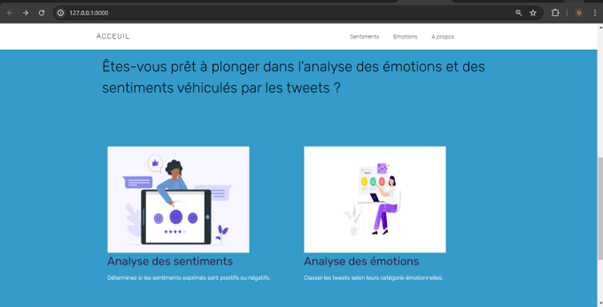
\includegraphics[width=0.9\linewidth]{project_report/figures/Acc2.png}
    \caption{\textit{Interface 1: Choix de type de saisie}}
    \label{fig:acc}
\end{figure}



\subsubsection{Interfaces d'importation des données}
\begin{figure}[h]
    \centering
    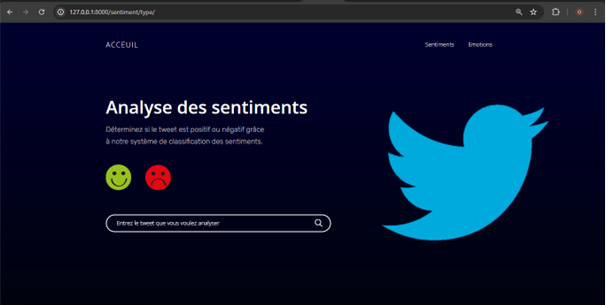
\includegraphics[width=0.9\linewidth]{project_report/figures/entrer un text.png}
    \caption{\textit{Interface 2: saisir un texte.}}
    \label{fig:text}
\end{figure}
Cette interface [\ref{fig:text}] offre à l'utilisateur la possibilité d'analyser les sentiments d'un texte. Voici les fonctionnalités qu'elle offre :
\begin{enumerate}
    \item \textbf{Zone de saisie de texte : }Si l'utilisateur choisit la saisie manuelle, il peut saisir un tweet ou tout autre texte dans cette zone dédiée. Cette fonctionnalité permet une analyse en temps réel des sentiments du texte saisi.
    \item \textbf{Bouton d'analyse :} Une fois que l'utilisateur a entré le texte, il peut cliquer sur ce bouton entrer pour lancer le processus d'analyse des sentiments. Après l'analyse, les résultats sont affichés à l'utilisateur.
    \item \textbf{Option d'importation de fichier :} Si l'utilisateur choisit d'importer un fichier, il peut cliquer sur cette option pour sélectionner un fichier texte contenant plusieurs tweets à analyser en une seule fois. Cela offre une flexibilité supplémentaire pour l'analyse de gros volumes de données.
\end{enumerate}
Pour le choix le l'analyse des émotions l'utilisateur peut aussi choisir le type de saisie (Voir la figure [\ref{fig:tem}]): 
\begin{figure}[h]
    \centering
    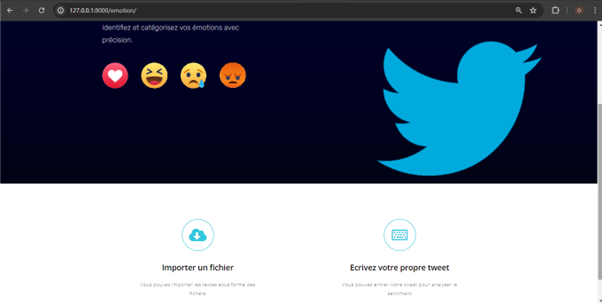
\includegraphics[width=0.9\linewidth]{project_report/figures/choix emotion.png}
    \caption{\textit{Interface 3: Choix de type de saisie.}}
    \label{fig:tem}
\end{figure}\\
Après que l'utilisateur a fait son choix concernant le type de saisie, les fonctionnalités de cette interface sont les mêmes que celles de l'analyse des sentiments. L'utilisateur peut soit entrer un texte manuellement dans la zone de saisie dédiée, soit importer un fichier (Voir la figure [\ref{fig:fechtt}]) contenant plusieurs textes à analyser. Dans les deux cas, l'utilisateur peut lancer l'analyse en cliquant sur le bouton entrer. Une fois l'analyse terminée, les résultats sont affichés de manière claire et concise, avec des visualisations graphiques et des statistiques détaillant les pourcentages de sentiments positifs et négatifs.
\begin{figure}[h]
    \centering
    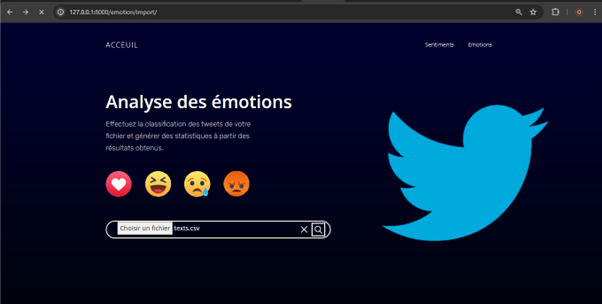
\includegraphics[width=0.9\linewidth]{project_report/figures/file.png}
    \caption{\textit{Interface 4: importer un fichier .}}
    \label{fig:fechtt}
\end{figure}
\subsection{Interface des resultats}
\begin{figure}[h]
    \centering
    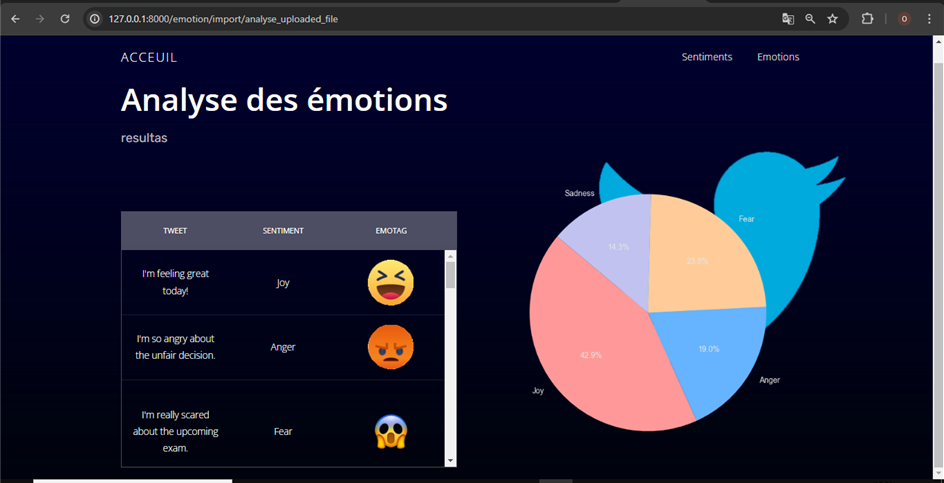
\includegraphics[width=0.9\linewidth]{project_report/figures/resultatsem.png}
    \caption{\textit{Interface 6: Résultat d'un fichier importé.}}
    \label{fig:emmmm}
\end{figure}
Pour les textes saisis, l'interface des résultats montre si le texte est positif ou négatif (Voir la figure [\ref{fig:sennnn}]), accompagné d'un emoji descriptif. Cela permet à l'utilisateur de comprendre rapidement l'émotion générale exprimée dans le texte de manière visuelle et intuitive.
\begin{figure}[h]
    \centering
    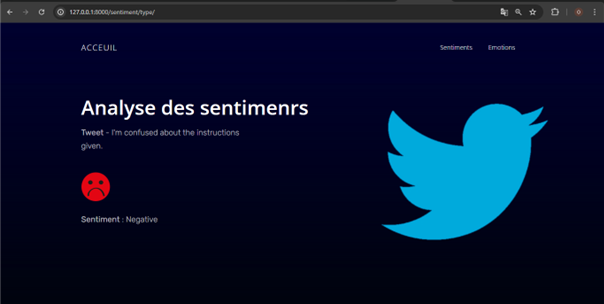
\includegraphics[width=0.9\linewidth]{project_report/figures/resultatssenn.png}
    \caption{\textit{Interface 5: Résultat d'un texte saisie.}}
    \label{fig:sennnn}
\end{figure}

Pour les fichiers importés, l'interface des résultats affiche un tableau détaillant les différentes sentiments et émotions prédites. En complément, un diagramme circulaire (pie chart) est présenté pour illustrer les statistiques des différentes émotions détectées dans l'ensemble du fichier (Voir la figure [\ref{fig:emmmm}]). Cette présentation visuelle offre une vue d'ensemble claire et facile à interpréter des émotions dominantes, facilitant l'analyse des données en masse.






\newpage


\textbf{Conclusion}\par
En conclusion, ce chapitre a présenté les résultats de notre projet, en mettant en évidence les performances des modèles et en comparant les résultats obtenus. Ces résultats fournissent des informations précieuses sur l'efficacité de nos approches et nous permettent de mieux comprendre les défis et les opportunités dans le domaine de l'analyse des sentiments et des émotions. Alors que nous continuons à développer notre projet et à explorer de nouvelles avenues de recherche, les résultats présentés dans ce chapitre serviront de base solide pour guider nos futurs efforts et initiatives dans ce domaine en constante évolution.




